\documentclass{article}
\usepackage[utf8]{inputenc}
\usepackage{amsmath}
\usepackage{graphicx}

\usepackage{titling}
\usepackage{hyperref}

\predate{\par\large\centering}
\postdate{\par}

\title{Gambleswap}
\author{Gambleswap Team}
\date{March 2022}

\begin{document}

\maketitle

\begin{abstract}

Gambleswap is a Constant Product Automated Market Making protocol. Liquidity providers will be given \$GMB as a form of passive income and may enter into a gambling game to bet with their \$GMBs. 
The chance of winning in the game is proportional to the \$GMBs each user has put in the game. Also, it's designed to have the ability to control the total supply and price of \$GMB.

\end{abstract}
\section{Decentralized Exchange}
As a fork of Uniswap, Gambleswap is, in its core, a decentralized liquidity pool based exchange. Liquidity pools contain a huge amounts of two different assets like $aToken$ and $bToken$. 
Users can use these pools to swap their $aTokens$ with $bTokens$ or vice versa. They deposit one token and take a a certain amount of the other token. The ratio between the amount of token a user deposits and the amount of the token they take out is calculated through an Automated Market Maker (AMM) which will be discussed more later.
Liquidity providers are users who deposit both tokens into the pool. As a reward they receive Liquidity Provider (LP) tokens. In Gambleswap, in addition to LP tokens, they also receive \$GMB. These tokens can be used to participate in the gambling. 
\section{Automated Market Maker}
As mentioned before there are two tokens in each liquidity pool in an AMM-based exchange. The ratio between the amount of one token a user takes out and the amount of the other token the user endows, are calculated using a formula. The purpose of the formula is to make sure the exchanges that happen in the pool do not impose a massive impact on the prices of the two tokens and the prices remain as stable as possible. Hence, the slippage of the pools remain low. 
The formula basically tries to keep the product of the amounts of the two tokens at a constant value $k$.
Assume the amounts of the tokens are $R_a$ and $R_b$ before the swap. A user can deposit $x$ tokens of $R_a$ in the pool and take $y$ tokens of $R_b$ out. 
A small portion of $x$ is taken as a fee. This fee is divided between all liquidity providers proportional to their share in the pool. The fee ratio is shown by $\mu$. Now, because the product of the two tokens amounts should remain equal to $k$, we can calculate $y$ like this:

\begin{align*}
    R_a R_b &= (R_a + (1 - \mu)x)(R_b - y) \\
    \to (1 - \mu)xR_b &= (1 - \mu)xy + yR_1 \\
    \to y &= R_b - \frac{R_aR_b}{R_a + (1 - \mu)x}
\end{align*}


\section{Tokenomics}

The new ERC20 token that we define and use in gambleswap, is called GMB. 
LP token holders will receive \$GMB as rewards. Later, they can use them to participate in the gambling.

\subsection{Mint GMB}

A fixed number of \$GMB is minted in each block. Each liquidity provider will receive a fraction of these tokens which is proportional to the amount of their LP tokens. In order to get these \$GMBs, the user needs to claim them. When a user $u$ claims that they should receive GMB tokens, we calculate the number of blocks that have been mined after their last claim and then find out their GMB tokens as follows:

$$
\text{ number of GMB tokens } u \text{ gets in a claim} =
$$
$$
\text{ number of blocks since } u \text{'s last claim}
$$
$$
\times \text{ number of GMB tokens minted every block}
$$
$$\times (\frac{\text{number of } u \text{'s LP tokens}}{\text{total LP tokens}})
$$

To make it easier for the users to receive their \$GMB, the pool contract automatically claims these tokens for them whenever they update their LP token value, i.e. when they deposit liquidity to or withdraw liquidity from the pool.


\subsection{Burn GMB}
To be able to control the price and value of \$GMB, we designed a process to burn some of the minted tokens on a regularly basis. We will discuss it in more details in the following sections.

\section{Gambling Game}
The gambling game is the powerful core of the enhancements added to the central uniswap logic. The rules of the game can be basically listed as follows:
\begin{itemize}
    \item Participants send their GMB tokens into the gambling contract. These tokens are accumulated to form our jackpot. They also send their bet values, which is a number they have guessed within a particular interval.
    \item A random number is generated using some properties of the block like block number, block difficulty, and block timestamp.
    \item If the number a user has bet on, falls inside a certain distance from the randomly generated number, that user is one of the winners of the game. This distance gets larger depending on the amount of GMB tokens they have deposited into the jackpot.
    \item 25 percent of the jackpot is burnt in each game. This is done in order to control the GMB total supply.
    \item If a game doesn't have any winners, the jackpot's contents remain in the jackpot and will be used in the next round. This gives motivation to users to participate in the game if they see there is non-empty jackpot before they start the game. Therefore, the number of participants can grow substantially. 
    \item Every fourth game, all the value in the jackpot gets burnt.
    \item Participants need to own some LP tokens to be able to play in the game. We lock their LP tokens during the game. This rule intends to motivate users to provide liquidity in our pools.
    \item After the game is over, users who have won, can claim their rewards and unlock their LP tokens. 
    \item Logs of all the past games are kept in our contract, so that users can claim any time they like.
    \item The maximum chance of winning is 50 percent. It means if a player owns all the \$GMBs in the jackpot, she or he has a maximum 50 percent chance of winning. 
\end{itemize}

\subsection{Determining winners}
We introduce a variable as $coveragePerGMB$. This value demonstrates the length of the interval that each GMB token covers. Participants can increase their coverage by having more GMBs in the game. The value $UserCoverage$ shows the maximum distance the user's bet value can have with the correct random number for the user to win. The greater this value, the more chance the user has for winning. This value is calculated as follows. 

\begin{align*}
    \text{user's coverage} &= min( \frac{1}{4} \times \text{maximum random number}, \\
    &\text{coveragePerGMB} \times \text{user's GMB tokens})
\end{align*}

the $\frac{1}{4} \times \text{maximum random number}$ is there to bound the maximum chance of winning to 50 percent.


The coveragePerGMB's value in each round is calculated based on the value of the jackpot in the previous game. For the first game we assume the coveragePerGMB value is 10, and for games after that we have:
$$
\text{ coveragePerGMB } = \frac{\text{maximum random number}}{\text{4}
\times \text{total jackpot of the previous game}}
$$


The coveragePerGMB is a dynamic value depending on the previous game. In each game, this value is the same for all users. Users have more chance to win by putting more GMB in the jackpot; each user wins if their bet value falls inside this interval:
$$
(\text{correct random number} - \text{user's coverage},$$
$$
\text{correct random number} + \text{user's coverage})
$$


If the number of participants in one game is small, the chance of winning in the next game goes higher; Consequently, more users are encouraged to participate in the next round. Figure \ref{fig:coverage} illustrates the process of determining the winners.


\begin{figure}
    \centering
    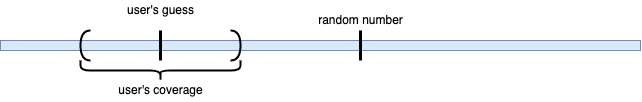
\includegraphics[width=\textwidth]{coverage.png}
    \caption{The blue interval shows the entire interval the random number can fall into. If the random number falls into the user's coverage, user will be one of the winners.}
    \label{fig:coverage}
\end{figure}

\subsection{Overflow/Underflow in the interval}
The generated interval for each user may exceed the $Maximum Random Number$ or may become less than $zero$. There are three scenarios for an interval:
\begin{itemize}
    \item Overflow: It happens when
    $$CorrectRandomNumber + UserCoverage > MaximumRandomNumber$$ In this scenario, the remaining  amount of the user's coverage will be considered from 0 to the OverflowValue. 
    
    \begin{align*}
        \text{OverflowValue} &= \text{UserCoverage} \\ &+ \text{CorrectRandomNumber} \\ &-  \text{MaxRandomNumber}
    \end{align*}
    
    Users  will win when the below condition holds:
    $$(\text{betValue} > (\text{correctRandomNumber} - \text{UserCoverage})$$
    $$\lor$$
    $$
     \text{betValue} < \text{overflowValue}
    $$
    
    \item Underflow: This happens when 
    $$UnderflowValue = UserInterval - CorrectRandomNumber$$
    Users  will win when the below condition holds:
    $$
    (\text{betValue} > (\text{maxRandomNumber} - \text{UnderflowValue}))
    $$
    $$\lor$$
    $$
     (\text{betValue} < (\text{CorrectRandomNumber} + \text{UserCoverage}))
    $$
    
    Figure \ref{fig:overflow} shows the coverage of the user in cases of underflow and overflow.
    
    \item Normal: In this scenario users will win when their $betValue$ is in the below interval:
    $$
    {CorrectRandomNumber \pm{UserInterval}}
    $$
\end{itemize}

\begin{figure}
    \centering
    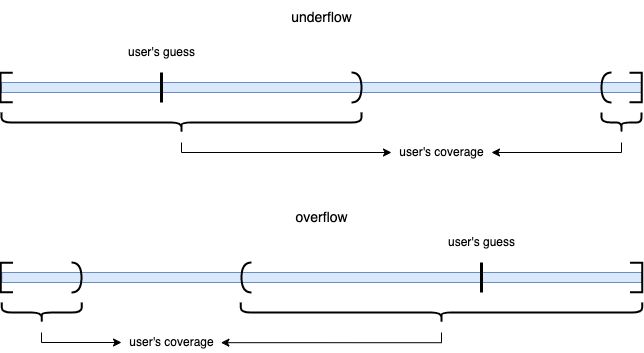
\includegraphics[width=\textwidth]{coverage2.png}
    \caption{User's coverage in underflow and overflow cases.}
    \label{fig:overflow}
\end{figure}

\subsection{Generating random number}
The random number in each game is calculated with a formula that considers these variables:
\begin{itemize}
    \item Block Timestamp
    \item Block Difficulty
    \item Block Number
    \item Admin address
\end{itemize}

\subsection{Expected value of net profit}

Let's assume user $u_i$ deposits $a_i$ GBM tokens in the gambling contract. The random number can be between zero and the maximum. Let's assume the maximum is $M$ and the number of participants is $n$ and number of winners is $W$. Also, $\frac{1}{4}$ of the tokens are burnt.
Therefore, the probability of $u_i$ being one of the winners is:
\begin{equation*}
    p_i = a_i \times \frac{1}{4\times (\sum_{i = 0}^{n} a_i)_{lastRound}}
\end{equation*}
Hence, the expected value of $u_i$'s profit in one round of gambling is:
\begin{align*}
    E[profit(u_i)] &= p_i \times \frac{3\sum_{i=0}^{n}a_i}{4W} \\
    &=
    a_i \times \frac{1}{4\times (\sum_{i = 0}^{n} a_i)_{lastRound}} \times 
    \frac{3\sum_{i=0}^{n}a_i}{4W} \\
    &= 
    \frac{a_i}{16 W} \times \frac{3\sum_{i=0}^{n} a_i}{(\sum_{i=0}^{n} a_i)_{lastRound}}
\end{align*}

As we see, when the number of players increases in one round in respect to the last round, the probability of winning increases. If we assume the 
$\frac{\sum_{i=0}^{n} a_i}{(\sum_{i=0}^{n} a_i)_{lastRound}}$ factor to be close to one, we can see that 

$$
E[profit(u_i)] \approx \frac{3a_i}{16W}
$$
So, the expected net profit of the the $u_i$ is approximately
$
\frac{3a_i}{16W} - a_i
$.


\section{Source}
the source code and wirefram can be found here:
\href{https://github.com/Gambleswap}{https://github.com/Gambleswap}



\end{document}
